% \documentclass[handout]{beamer}
\documentclass{beamer}

\mode<presentation>
{
  \usetheme{default}
  \usefonttheme[onlymath]{serif}
  % \usetheme{Singapore}
  % \usetheme{Warsaw}
  % \usetheme{Malmoe}
  % \useinnertheme{circles}
  % \useoutertheme{infolines}
  % \useinnertheme{rounded}

  \setbeamercovered{transparent=100}
}

\usepackage[english]{babel}
\usepackage[latin1]{inputenc}
\usepackage{alltt,listings,multirow,ulem,siunitx}
\usepackage[absolute,overlay]{textpos}
\TPGrid{1}{1}
\usepackage{pdfpages}
\usepackage{multimedia}
\usepackage{multicol}
\newcommand\hmmax{0}
\newcommand\bmmax{0}
\usepackage{bm}

% font definitions, try \usepackage{ae} instead of the following
% three lines if you don't like this look
\usepackage{mathptmx}
\usepackage[scaled=.90]{helvet}
% \usepackage{courier}
\usepackage[T1]{fontenc}
\usepackage{tikz}
\usetikzlibrary{decorations.pathreplacing}
\usetikzlibrary{shadows,arrows,shapes.misc,shapes.arrows,shapes.multipart,arrows,decorations.pathmorphing,backgrounds,positioning,fit,petri,calc,shadows,chains,matrix}


% \usepackage{pgfpages}
% \pgfpagesuselayout{4 on 1}[a4paper,landscape,border shrink=5mm]

\usepackage{JedMacros}

\title{Low-memory low-communication multigrid}
\subtitle{Compression and resilience}
\author{Mark Adams\inst{1} and Jed Brown\inst{2}}

% - Use the \inst command only if there are several affiliations.
% - Keep it simple, no one is interested in your street address.
\institute
{
  \inst{1}{Columbia University}
  \inst{2}{Mathematics and Computer Science Division, Argonne National Laboratory} \\
}

\date{Argonne National Laboratory, 2012-10-19}

% This is only inserted into the PDF information catalog. Can be left
% out.
\subject{Talks}


% If you have a file called "university-logo-filename.xxx", where xxx
% is a graphic format that can be processed by latex or pdflatex,
% resp., then you can add a logo as follows:

% \pgfdeclareimage[height=0.5cm]{university-logo}{university-logo-filename}
% \logo{\pgfuseimage{university-logo}}



% Delete this, if you do not want the table of contents to pop up at
% the beginning of each subsection:
% \AtBeginSubsection[]
% {
% \begin{frame}<beamer>
%   \frametitle{Outline}
%   \tableofcontents[currentsection,currentsubsection]
% \end{frame}
% }

\AtBeginSection[]
{
  \begin{frame}<beamer>
    \frametitle{Outline}
    \tableofcontents[currentsection]
  \end{frame}
}

% If you wish to uncover everything in a step-wise fashion, uncomment
% the following command:

% \beamerdefaultoverlayspecification{<+->}

\begin{document}
\lstset{language=C}
\normalem

\begin{frame}
  \titlepage
\end{frame}

\begin{frame}
  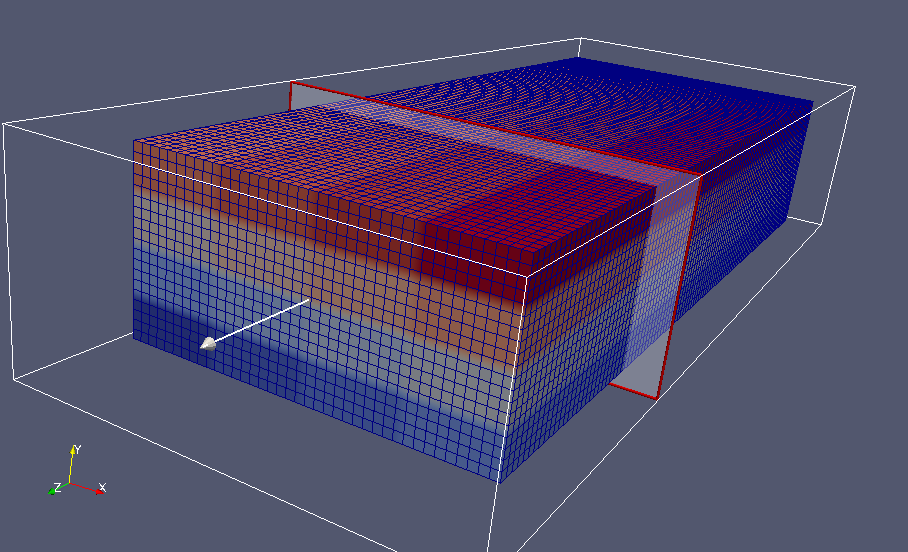
\includegraphics[width=\textwidth]{figures/MGSlice}
  \begin{itemize}
  \item Sweep through ``coarse'' grid with moving window
  \item Zoom in on new slab, construct fine grid ``window'' in-cache
  \item Interpolate to new fine grid, apply pipelined smoother ($s$-step)
  \item Compute residual, accumulate restriction of state and residual into coarse grid, expire slab from window
  \end{itemize}
\end{frame}

\begin{frame}{Basic resilience strategy}
  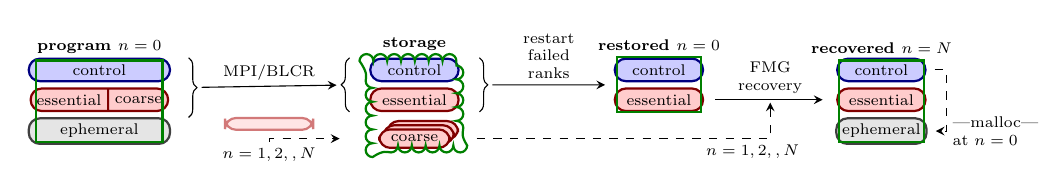
\begin{tikzpicture}
    [scale=0.8,every node/.style={scale=0.8},
    >=stealth,
    control/.style={rectangle,rounded corners,draw=blue!50!black,fill=blue!20,thick,minimum width=5em},
    essential/.style={rectangle,rounded corners,draw=red!50!black,fill=red!20,thick,minimum width=5em},
    ephemeral/.style={rectangle,rounded corners,draw=gray!50!black,fill=gray!20,thick,minimum width=5em},
    statebox/.style={rectangle,draw=green!50!black,thick},
    statetitle/.style={rectangle,draw=green!50!black,fill=green!20,thick},
    storebox/.style={rectangle,draw=},
    rightbrace/.style={decorate,decoration={brace,amplitude=1ex,raise=4pt}},
    leftbrace/.style={decorate,decoration={brace,amplitude=1ex,raise=4pt,mirror}}
    ]
    \scriptsize
    \node[control,minimum width=8em] (progcontrol) {control};
    \node[essential,below=2pt of progcontrol.south,rectangle split,rectangle split parts=2,rectangle split horizontal,minimum width=12em] (progessential) {essential \nodepart{two} coarse};
    \node[ephemeral,minimum width=8em,below=2pt of progessential.south] (progephemeral) {ephemeral};
    \node[statebox,fit=(progcontrol)(progessential)(progephemeral)] (progbox) {};
    \node[above=0pt of progbox.north,anchor=south] {\textbf{program $n=0$}};

    \node[control,right=9em of progcontrol] (storecontrol) {control};
    \node[essential,below=2pt of storecontrol.south] (storeessential) {essential};
    \node[essential,minimum width=4em,below=6pt of storeessential.south, double copy shadow] (storecoarse) {coarse};
    \node[statebox,decorate,decoration={bumps,mirror},fit=(storecontrol)(storecoarse)] (storebox) {};
    \node[above=1pt of storebox.north,anchor=south] {\textbf{storage}};

    \node[control,right=7em of storecontrol] (reccontrol) {control};
    \node[essential,below=2pt of reccontrol.south] (recessential) {essential};
    \node[statebox,fit=(reccontrol)(recessential)] (recbox) {};
    \node[above=0pt of recbox.north,anchor=south] {\textbf{restored $n=0$}};

    \node[control,right=6em of reccontrol] (donecontrol) {control};
    \node[essential,below=2pt of donecontrol.south] (doneessential) {essential};
    \node[ephemeral,below=2pt of doneessential.south] (doneephemeral) {ephemeral};
    \node[statebox,fit=(donecontrol)(doneephemeral)] (donebox) {};
    \node[above=0pt of donebox.north,anchor=south] {\textbf{recovered $n=N$}};

    \draw[decorate,decoration={brace,amplitude=1ex,raise=4pt}] ($(progcontrol.north east) + (3pt,0)$) -- ($(progephemeral.north east) + (3pt,0)$) node[midway,xshift=1ex] (progbrace) {};
    \draw[leftbrace] ($(storecontrol.north west) - (4pt,0)$) -- ($(storeessential.south west) - (4pt,0)$) node[midway,xshift=-1ex] (storebrace) {};
    \draw[rightbrace] ($(storecontrol.north east) + (4pt,0)$) -- ($(storeessential.south east) + (4pt,0)$) node[midway,xshift=1ex] (storerbrace) {};
    \draw[->,shorten >=4pt,shorten <=4pt] (progbrace) -- (storebrace) node[midway,above] (midarrow) {MPI/BLCR};

    \node[below=1.4em of midarrow,essential,draw=red!50!gray!70,fill=red!10] (coarserun) {};
    \draw[->,dashed,shorten >=14pt,shorten <=4pt] (coarserun) |- (storecoarse) node [near start,below,yshift=-3pt] {\scriptsize $n=1,2,\dotsc,N$};
    \draw[->,shorten >=4pt,shorten <=4pt] (storerbrace) -- (recbox.west) node[midway,above,text width=5em,align=center] (midarrow) {restart failed ranks};
    \draw[->,shorten >=5pt,shorten <=4pt] (recessential.east) -- (doneessential) node[midway,above,text width=5em,align=center] (fmgrecover) {FMG recovery};
    \draw[->,dashed,shorten >=1pt,shorten <=3pt] ($(storecoarse.east) + (1em,0)$) -| (fmgrecover) node[midway,below,xshift=-1em] {\scriptsize $n=1,2,\dotsc,N$};
    \draw[->,dashed,shorten >=3pt,shorten <=3pt] (donecontrol.east) -| ($(donecontrol.east) + (3ex,0)$) |- (doneephemeral.east) node[midway,right,text width=4em] {\cverb|malloc| at $n=0$};
  \end{tikzpicture}
\begin{description}
\item[control] contains program stack, solver configuration, etc.
\item[essential] program state that cannot be easily reconstructed: time-dependent solution, current optimization/bifurcation iterate
\item[ephemeral] easily recovered structures: assembled matrices, preconditioners, residuals, Runge-Kutta stage solutions
\end{description}
\begin{itemize}
\item Essential state at time/optimization step $n$ is \alert{inherently globally coupled} to step $n-1$ (otherwise we could use an explicit method)
\item \emph{Coarse} level checkpoints are orders of magnitude smaller, but allow rapid recovery of essential state
\item FMG recovery needs only \alert{nearest neighbors}
\end{itemize}
\end{frame}

\newcommand{\timeR}{t_{\mathrm{R}}}
\newcommand{\timeW}{t_{\mathrm{W}}}
\newcommand{\mglevel}{\ensuremath{\ell}}
\newcommand{\mglevelcp}{\ensuremath{\mglevel_{\mathrm{cp}}}}
\newcommand{\mglevelfine}{\ensuremath{\mglevel_{\mathrm{fine}}}}
\begin{frame}[fragile]{Multiscale compression and recovery using $\tau$ form}
   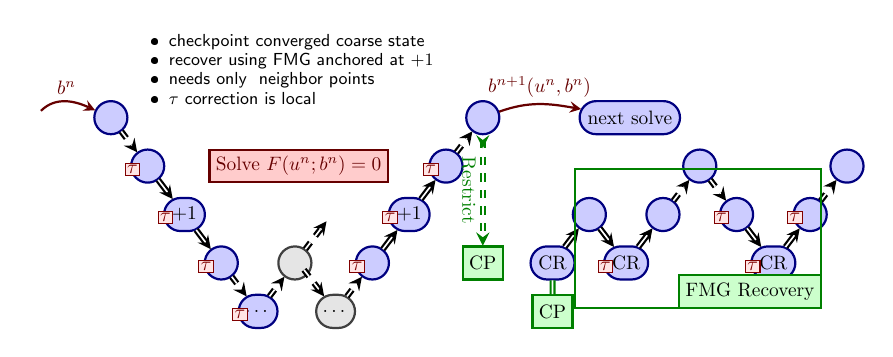
\begin{tikzpicture}
    [scale=0.7,every node/.style={scale=0.7},
    >=stealth,
    restrict/.style={thick,double},
    prolong/.style={thick,double},
    cprestrict/.style={green!50!black,thick,double,dashed},
    control/.style={rectangle,red!40!black,draw=red!40!black,thick},
    mglevel/.style={rounded rectangle,draw=blue!50!black,fill=blue!20,thick,minimum size=6mm},
    checkpoint/.style={rectangle,draw=green!50!black,fill=green!20,thick,minimum size=6mm},
    mglevelhide/.style={rounded rectangle,draw=gray!50!black,fill=gray!20,thick,minimum size=6mm},
    tau/.style={text=red!50!black,draw=red!50!black,fill=red!10,inner sep=1pt},
    crelax/.style={text=green!50!black,fill=green!10,inner sep=0pt}
    ]
    \begin{scope}
      \newcommand\mgdx{1.9em}
      \newcommand\mgdy{2.5em}
      \newcommand\mgloc[4]{(#1 + #4*\mgdx*#3,#2 + \mgdy*#3)}
      \node[mglevel] (fine0) at \mgloc{0}{0}{4}{-1} {\mglevelfine};
      \node[mglevel] (finem1down0) at \mgloc{0}{0}{3}{-1} {};
      \node[mglevel] (cp1down0) at \mgloc{0}{0}{2}{-1} {$\mglevelcp+1$};
      \node[mglevel] (cpdown0) at \mgloc{0}{0}{1}{-1} {\mglevelcp};
      \node[mglevel] (coarser0) at \mgloc{0}{0}{0}{0} {\ldots};

      \node[mglevelhide] (cpup0) at \mgloc{0}{0}{1}{1} {};
      \node (cp1up0) at \mgloc{0}{0}{2}{1} {};

      \node (cpdown1) at \mgloc{4em}{0}{1}{-1} {};
      \node[mglevelhide] (coarser1) at \mgloc{4em}{0}{0}{1} {\ldots};
      \node[mglevel] (cpup1) at \mgloc{4em}{0}{1}{1} {\mglevelcp};
      \node[mglevel] (cp1up1) at \mgloc{4em}{0}{2}{1} {$\mglevelcp+1$};
      \node[mglevel] (finem1up1) at \mgloc{4em}{0}{3}{1} {};
      \node[mglevel] (fine1) at \mgloc{4em}{0}{4}{1} {\mglevelfine};

      \draw[->,restrict,dashed] (fine0) -- (finem1down0);
      \draw[->,restrict] (finem1down0) -- (cp1down0);
      \draw[->,restrict] (cp1down0) -- (cpdown0);
      \draw[->,restrict,dashed] (cpdown0) -- (coarser0);
      \draw[->,prolong,dashed] (coarser0) -- (cpup0);
      \draw[->,prolong,dashed] (cpup0) -- (cp1up0);

      \draw[->,restrict,dashed] (cpdown1) -- (coarser1);
      \draw[->,prolong,dashed] (coarser1) -- (cpup1);
      \draw[->,prolong] (cpup1) -- (cp1up1);
      \draw[->,prolong] (cp1up1) -- (finem1up1);
      \draw[->,prolong,dashed] (finem1up1) -- (fine1);

      \node[checkpoint] at (4em + \mgdx*4,\mgdy) (cp) {CP};
      \draw[>->,cprestrict] (fine1) -- node[below,sloped] {Restrict} (cp);

      \node[left=\mgdx of fine0] (bnanchor) {};
      \node[control,fill=red!20] at (1.1*\mgdx,3*\mgdy) {Solve $F(u^n;b^n) = 0$};
      \node[mglevel,right=of fine1] (finedt) {next solve};
      \draw[->, >=stealth, control] (fine1) to[out=20,in=170] node[above] {$b^{n+1}(u^n,b^n)$} (finedt);
      \draw[->, >=stealth, control] (bnanchor) to[out=45,in=155] node[above] {$b^n$} (fine0);

      % Recovery process
      \begin{scope}[xshift=8*\mgdx]
        \node[checkpoint] (rcp) at \mgloc{0}{0}{0}{0} {CP};
        \node[mglevel] (r0a) at \mgloc{0}{\mgdy}{0}{0} {CR};
        \node[mglevel] (r1a) at \mgloc{0}{\mgdy}{1}{1} {};
        \node[mglevel] (r0b) at \mgloc{2*\mgdx}{\mgdy}{0}{0} {CR};
        \node[mglevel] (r1b) at \mgloc{2*\mgdx}{\mgdy}{1}{1} {};
        \node[mglevel] (r2b) at \mgloc{2*\mgdx}{\mgdy}{2}{1} {\mglevelfine};
        \node[mglevel] (r1c) at \mgloc{6*\mgdx}{\mgdy}{1}{-1} {};
        \node[mglevel] (r0d) at \mgloc{6*\mgdx}{\mgdy}{0}{0} {CR};
        \node[mglevel] (r1d) at \mgloc{6*\mgdx}{\mgdy}{1}{1} {};
        \node[mglevel] (r2d) at \mgloc{6*\mgdx}{\mgdy}{2}{1} {\mglevelfine};

        \draw[-,prolong,green!50!black] (rcp) -- (r0a);
        \draw[->,prolong] (r0a) -- (r1a);
        \draw[->,restrict] (r1a) -- (r0b);
        \draw[->,restrict] (r0b) -- (r1b);
        \draw[->,restrict,dashed] (r1b) -- (r2b);
        \draw[->,restrict,dashed] (r2b) -- (r1c);
        \draw[->,restrict] (r1c) -- (r0d);
        \draw[->,restrict] (r0d) -- (r1d);
        \draw[->,restrict,dashed] (r1d) -- (r2d);

        \foreach \smooth in {finem1down0, cp1down0, cpdown0, coarser0,
          cpup1, cp1up1, finem1up1,
          r0b,r1c,r0d,r1d} {
          \node[above left=-5pt of \smooth.west,tau] {$\tau$};
        }
        \node[rectangle,fill=none,draw=green!50!black,thick,fit=(rcp)(r2d)] (recoverbox) {};
        \node[rectangle,draw=green!50!black,fill=green!20,thick,minimum size=6mm,above={0cm of recoverbox.south east},anchor=south east] (recover) {FMG Recovery};
      \end{scope}
      \node (notation) at (\mgdx,5*\mgdy) {
        \begin{minipage}{18em}\small\sf
          \begin{itemize}\addtolength{\itemsep}{-5pt}
          \item checkpoint converged coarse state
          \item recover using FMG anchored at $\mglevelcp+1$
          \item needs only $\mglevelcp$ neighbor points
          \item $\tau$ correction is local
          \end{itemize}
        \end{minipage}
      };
    \end{scope}
  \end{tikzpicture}
  \begin{itemize}
  \item Normal multigrid cycles visit all levels moving from $n \to n+1$
  \item FMG recovery only accesses levels finer than $\ell_{CP}$
  \item Only failed processes and neighbors participate in recovery
  \item Lightweight checkpointing for transient adjoint computation
  \item Postprocessing applications, e.g., in-situ visualization at high temporal resolution in part of the domain
  \end{itemize}
\end{frame}
% \begin{frame}{$\tau$ formulation of Full Approximation Scheme (FAS)}
  \begin{itemize}
  \item classical formulation: ``coarse grid \emph{accelerates} fine grid $\searrow \nearrow$
  \item $\tau$ formulation: ``fine grid feeds back into coarse grid'' $\nearrow \searrow$
  \item To solve $N u = f$, recursively apply
    \begin{equation*}
      \begin{split}
        \text{pre-smooth} \:\: & \quad \tilde u^h \gets S^h_{\text{pre}}(u^h_0, f^h) \\
        \text{solve coarse problem for $u^H$} \:\: & \quad N^H u^H = \underbrace{I_h^H f^h}_{f^H} + \underbrace{N^H \hat I_h^H \tilde u^h - I_h^H N^h \tilde u^h}_{\tau_h^H} \\
        \text{correction and post-smooth} \:\: & \quad u^h \gets S^h_{\text{post}} \Big( \tilde u^h + I_H^h (u^H - \hat I_h^H \tilde u^h), f^h \Big) \\
      \end{split}
    \end{equation*}
    \begin{tabular}{llll}
      \toprule
      $I_h^H$ & residual restriction & $\hat I_h^H$ & solution restriction \\
      $I_H^h$ & solution interpolation & $f^H = I_h^H f^h$ & restricted forcing \\
      $\{S^h_{\text{pre}},S^h_{\text{post}}\}$ & \multicolumn{3}{l}{smoothing operations on the fine grid} \\
      \bottomrule
    \end{tabular}
  \item At convergence, $u^{H*} = \hat I_h^H u^{h*}$ solves the $\tau$-corrected coarse grid equation
    $N^H u^H = f^H + \tau_h^H$,
    thus $\tau_h^H$ is the ``fine grid feedback'' that makes the coarse grid equation accurate.
  \item $\tau_h^H$ is \emph{local} and need only be recomputed where it becomes stale.
  \end{itemize}
\end{frame}

% \begin{frame}{Cool Topics in Multiscale Computation}
  \begin{multicols}{2}
    \begin{itemize}
    \item Solve PDE in fewer flops than evaluating an analytic solution
    \item Solve PDE in $\bigO(\abs{\log n}\abs{\log \epsilon}^d)$ memory
    \item Compute $k$ eigenvalues in $\bigO(n \log k)$
    \item Project vector onto eigenbasis in $\bigO(n \log k)$
    \item Optimal-order graph partitioning and clustering
    \item Continuation and transient problems without revisiting fine grid
    \item Global optimization without sacrificing optimality, ``multiscale annealing''
    \item Accelerate Monte-Carlo slowdown due to spuriously correlated sampling
    \end{itemize}
  \end{multicols}
\end{frame}


\end{document}
